\documentclass[a4paper, 11pt]{article}

%% Language and font encodings
\usepackage[francais]{babel}
\usepackage[utf8x]{inputenc}
\usepackage[T1]{fontenc}

%% Sets page size and margins
\usepackage[a4paper,margin=1in]{geometry}

%% Useful packages
\usepackage{amsmath}
\usepackage{graphicx}
\usepackage[colorinlistoftodos]{todonotes}
\usepackage[colorlinks=true, allcolors=blue]{hyperref}
\usepackage{listings}
\usepackage{subfig}
\usepackage{color,soul}
\usepackage{hyperref}
\hypersetup{
     colorlinks   = true,
     linkcolor    = black
}
\usepackage{float}
\usepackage{multicol}

\setlength{\belowcaptionskip}{10pt}
\setlength{\parskip}{1em}
\newcommand{\hlc}[2][yellow]{{\sethlcolor{#1} \hl{#2}}}

\setcounter{tocdepth}{1}

\title{Vulptool}
\author{Aurélie Levy \and Miguel Pumbo Dias \and Valentin Finini \and Lawrence Stalder}

\begin{document}
\maketitle

\section{Description}
\subsection{Préface}
Ce projet répond au besoin de gestion de la part du chef de guilde afin de l'assister dans son travail de prévision des différentes soirées de jeu. L'object est de créer une interface simple pour que les membres de la guilde puissent s'inscrire à un evenement et que tous le monde puisse voir l'état (la présence) pour une soirée de raid.

\subsection{But}
Le but de se projet est de crée un site interet qui répond au besoin d'une guilde. Voici une liste non-exhaustive des fonctionnalités:

	\begin{enumerate}
		\item Afficher un calendrier
		\item Créer des raids (évenements)
		\item Créer des évenements enfant (ex: un par boss)
		\item Ajouter/Inviter des joueurs
		\item Trier les joueurs dans des roster (sous groupes)
		\item Authentification au moyen du service OAuth fourni par Blizzard
		\item Accepter/Refuser une invitation à une soirée de raid
		\item Tenir un journal (log) des évenements passés
		\item Créer des réglages prédéfinit et les réutiliser
		\item D'autres fonctionnalités liées au jeu World of Warcraft à proprement parlé
	\end{enumerate}

\subsection{Technologies}
Pour réaliser ce projet nous devons utiliser:
	
	\begin{enumerate}
		\item Scala Play
		\item Slik
		\item OAuth (fournit par Blizzard)
	\end{enumerate}

\subsection{Evénement}
Un événement, un raid, est un regroupement de plusieurs informations comme la date, l'heure, le raid concernés, le(s) boss concernés, les joueurs invités, leur status (Disponible, Indisponible, Confirmé, En attente, Disponible si besoin, Refusé). 

Le chef de guilde a un role d'administrateur et peut changer n'importe quelle information à n'importe quel moment. Les joueurs sont de simple utilisateurs, ils ont accès en lecture à toutes les informations mais peuvent modifier uniquement ce qui les concernes.

\subsection{REST API}
Afin de proposer un design évolutif et modifiable par la suite, nous allons implémenter notre site sur la base d'une API REST. Le frontend sera réaliser en React en éffectuant des requètes sur l'Api pour afficher les différents contenus. De cette manière nous espèront pouvoir, dans un deuxième temps (après le rendu du projet pour le cours Scala) améliorer le design du site internet.

\subsection{Pages}
Le site internet va comporter un minimum de deux pages disctinctes, la première affichera un calendrier avec les événements prévus pour la semaine à venir, une liste des membres de la guilde ainsi que des options. La deuxième page sera une répresentation d'une soirée en détails, avec l'affichage des joueurs et leurs status pour l'événement concerné. Il se peut que cette page soit un onglet dynamique ajouté à la page de base. 

En plus de ces deux visualisations, nous auront forcément une page de garde, une page de connexion, une page de gestion des personnages.

\subsection{Schéma BD}
La base de donnée de Vulptool suit ce le schéma en figure \ref{fig:DB}.

    \begin{figure}[ht]
        \center
        \frame{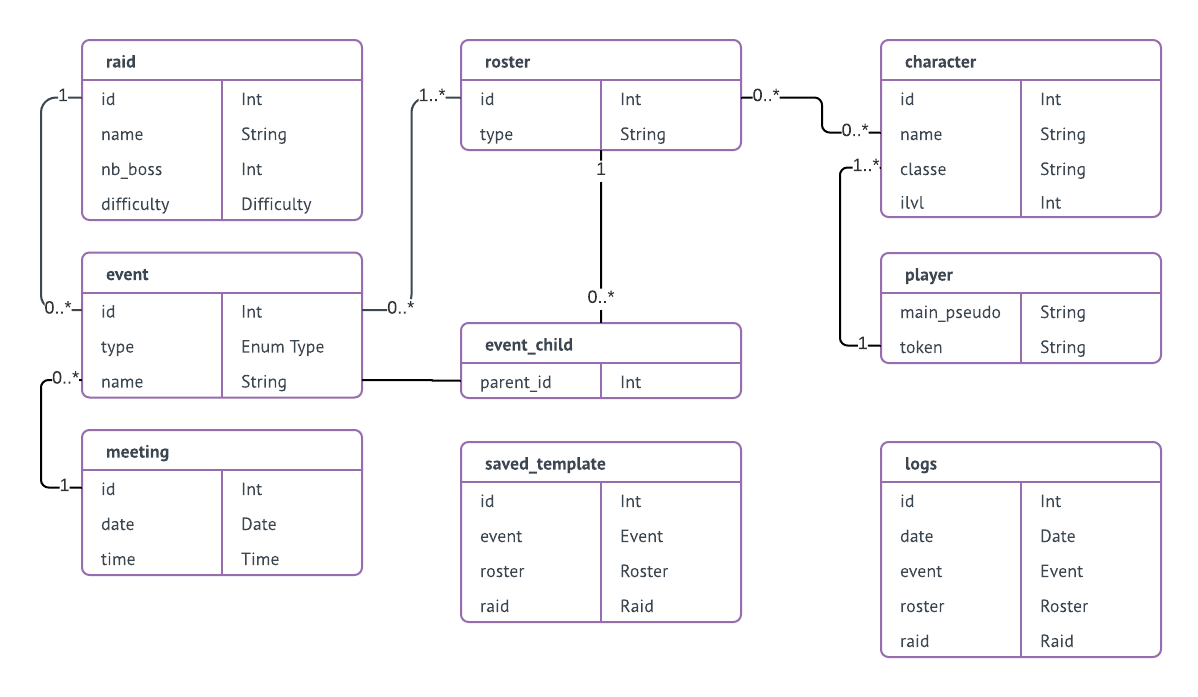
\includegraphics[width=\textwidth]{vulptoolDB.png}}
        \caption{Schéma Base de Donnée}
        \label{fig:DB}
    \end{figure}

    
  

\end{document}